\chapter{Conclusion}

% - Recall contributions with more details assuming someone has read it
%
% - Future work (chapter by chapter)
\section{Contributions}

In this thesis, we have developed some tools to better understand and make use
of the computations happening within complex systems.

\section{Future Work}

\subsection{Practical complexity}

\subsection{Feedback reservoir computing}

In Chapter \ref{cha:learn-effic-compl}, we explored the application
\begin{figure}[htbp]
  \centering
  \begin{subfigure}[t]{.5\linewidth}
    \centering
    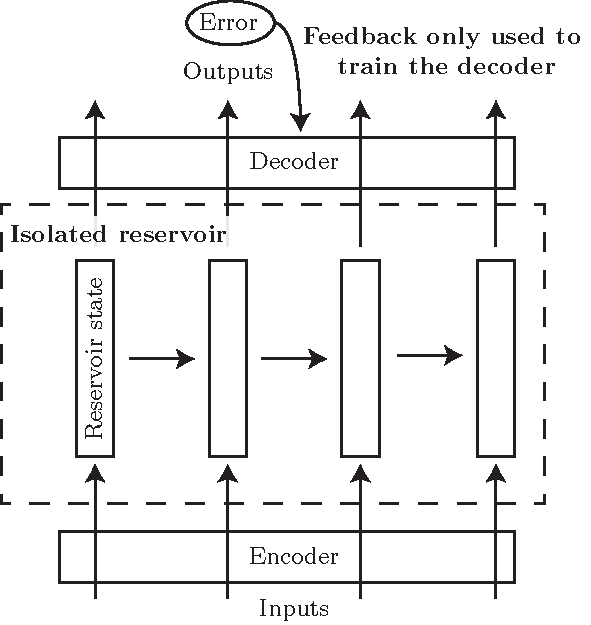
\includegraphics[width=\linewidth]{figures/classical_reservoir.pdf}
    \caption{Classical reservoir computing}
    \label{fig:classical_reservoir}
  \end{subfigure}
  \begin{subfigure}[t]{.45\linewidth}
    \centering
    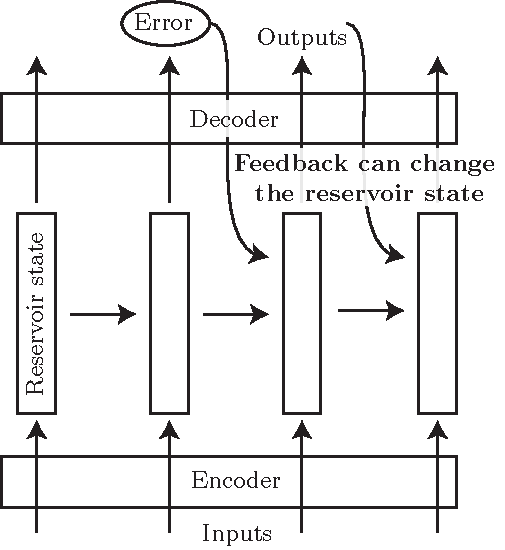
\includegraphics[width=\linewidth]{figures/feedback_reservoir.pdf}
    \caption{Feedback reservoir computing}
    \label{fig:feedback_reservoir}
  \end{subfigure}
  \caption{Comparison of regular reservoir computing with feedback reservoir computing}
  \label{"waiting for reftex-label call..."}
\end{figure}
